\chapter{Additional Material for \cref*{cha:mva}}\label{cha:appendix_mva}

\section{Observables used in the optimizattion}\label{app:mva:fulllistvars}

TODO

\section{KS-Test Correlation Plots}

\begin{figure}[htb]
    \centering
    \begin{subfigure}[t]{0.45\textwidth}
        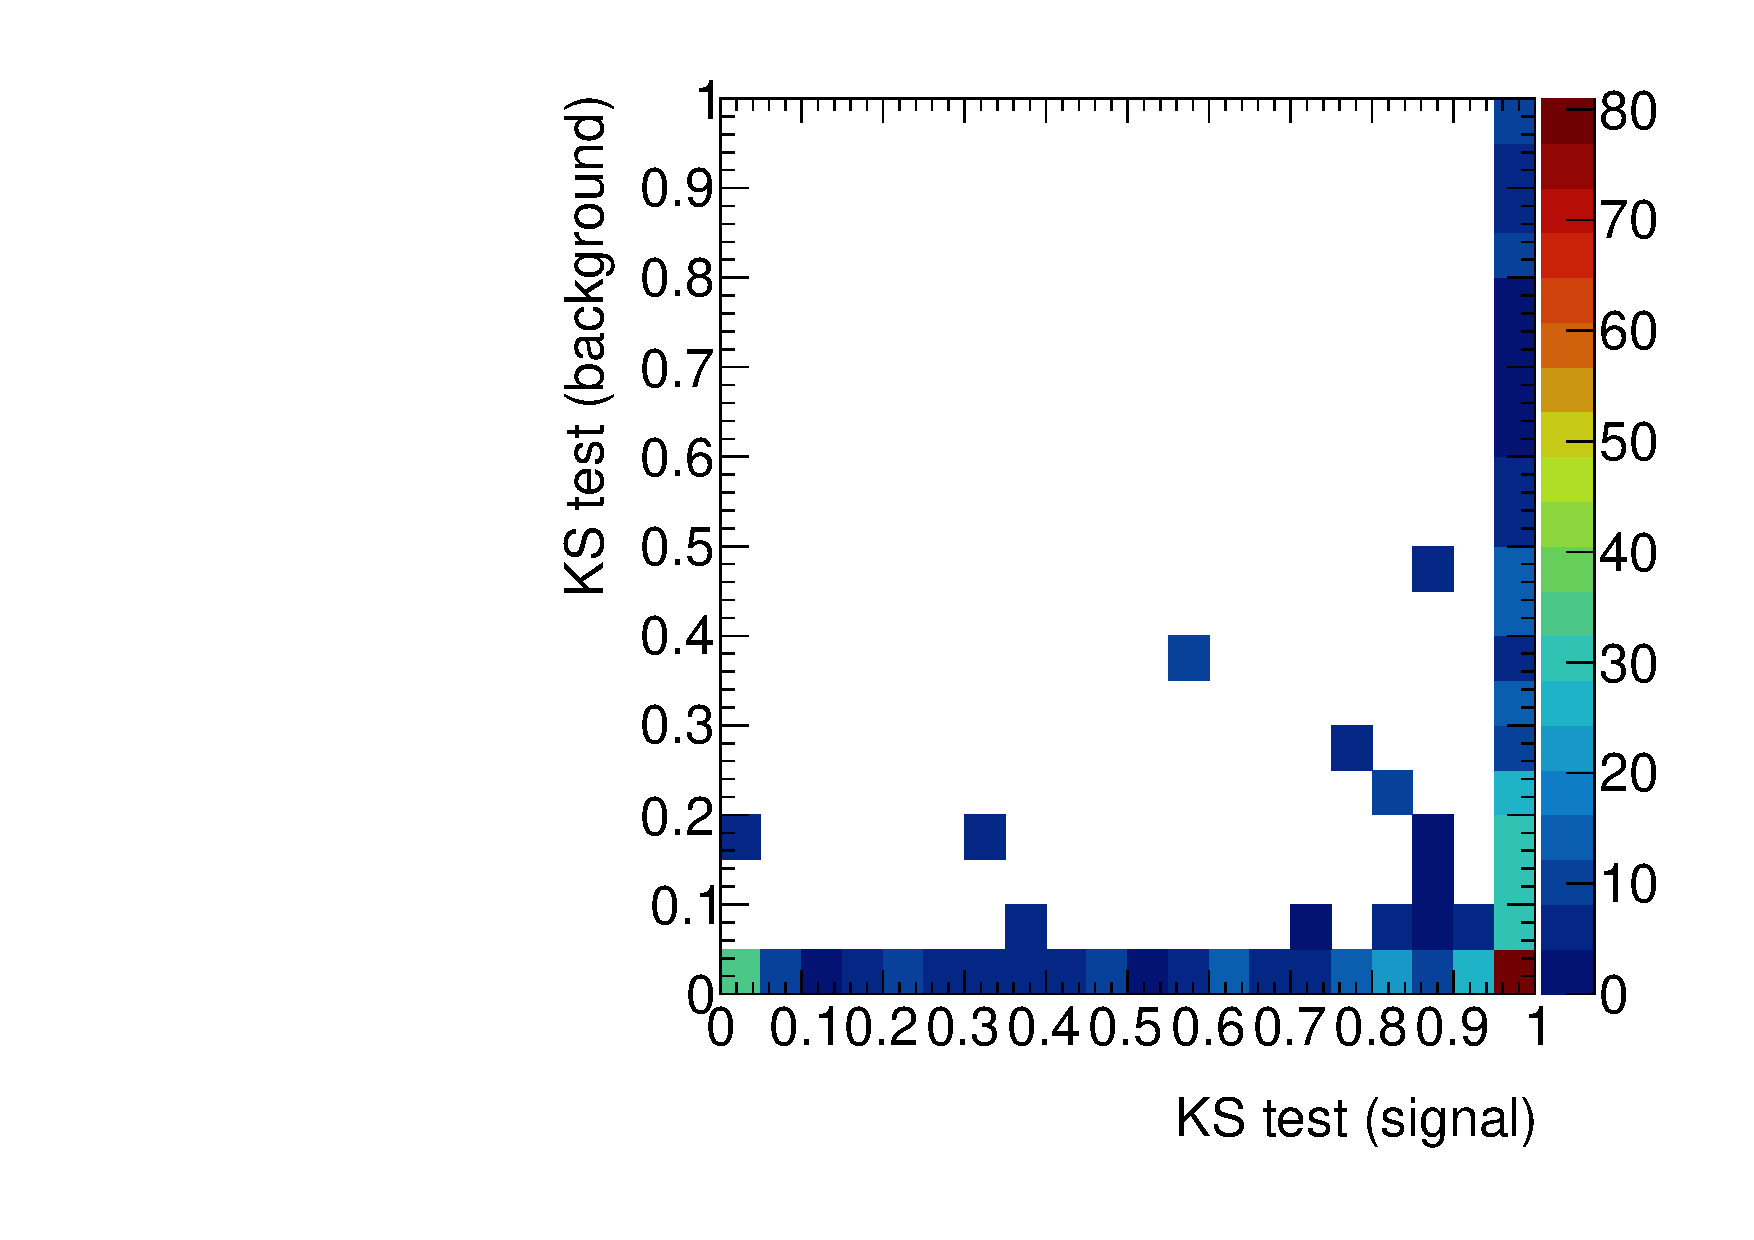
\includegraphics[width=\textwidth]{./plots/mva/scan/VBF_SF_ks_test_sig_vs_bkg.pdf}
        \caption{VBF SF}
    \end{subfigure}
    \begin{subfigure}[t]{0.45\textwidth}
        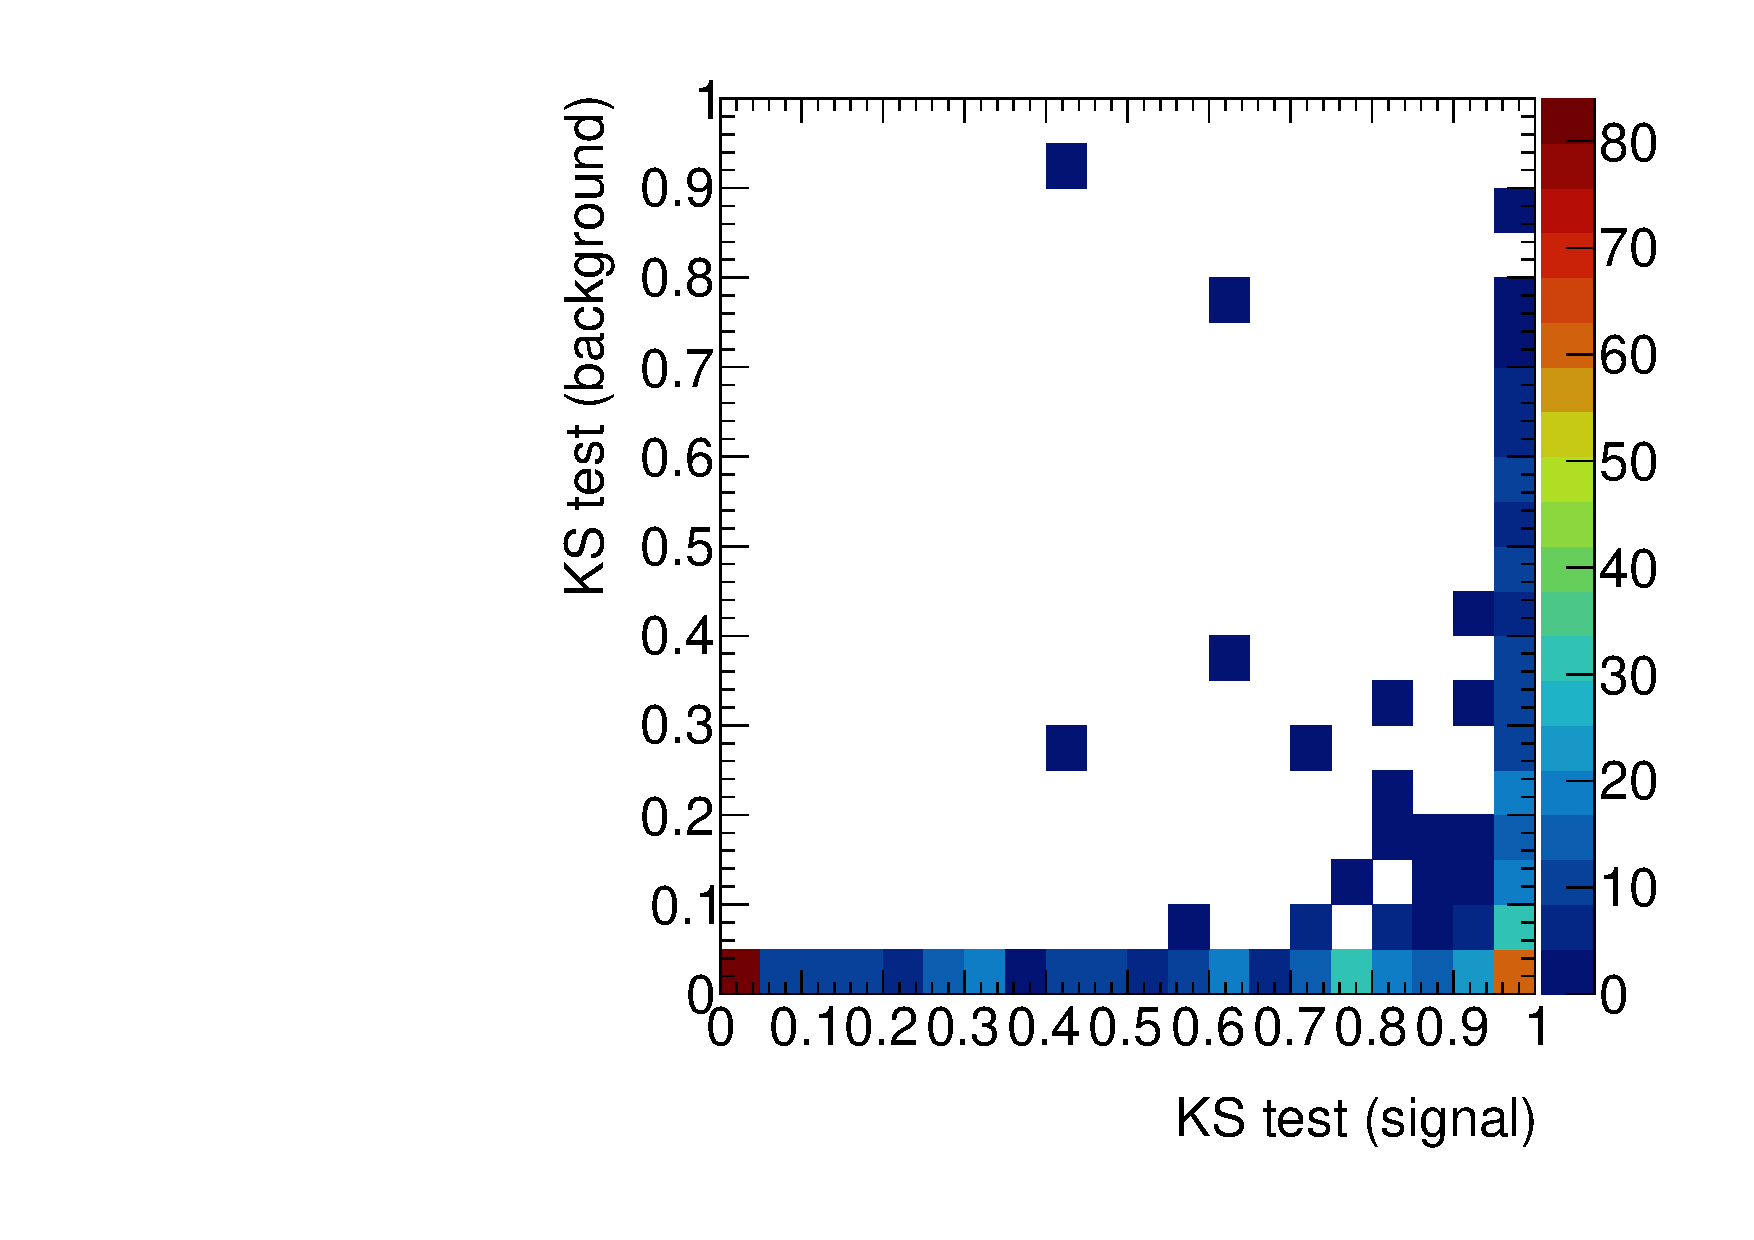
\includegraphics[width=\textwidth]{./plots/mva/scan/VBF_DF_ks_test_sig_vs_bkg.pdf}
        \caption{VBF DF}
    \end{subfigure}
    \begin{subfigure}[t]{0.45\textwidth}
        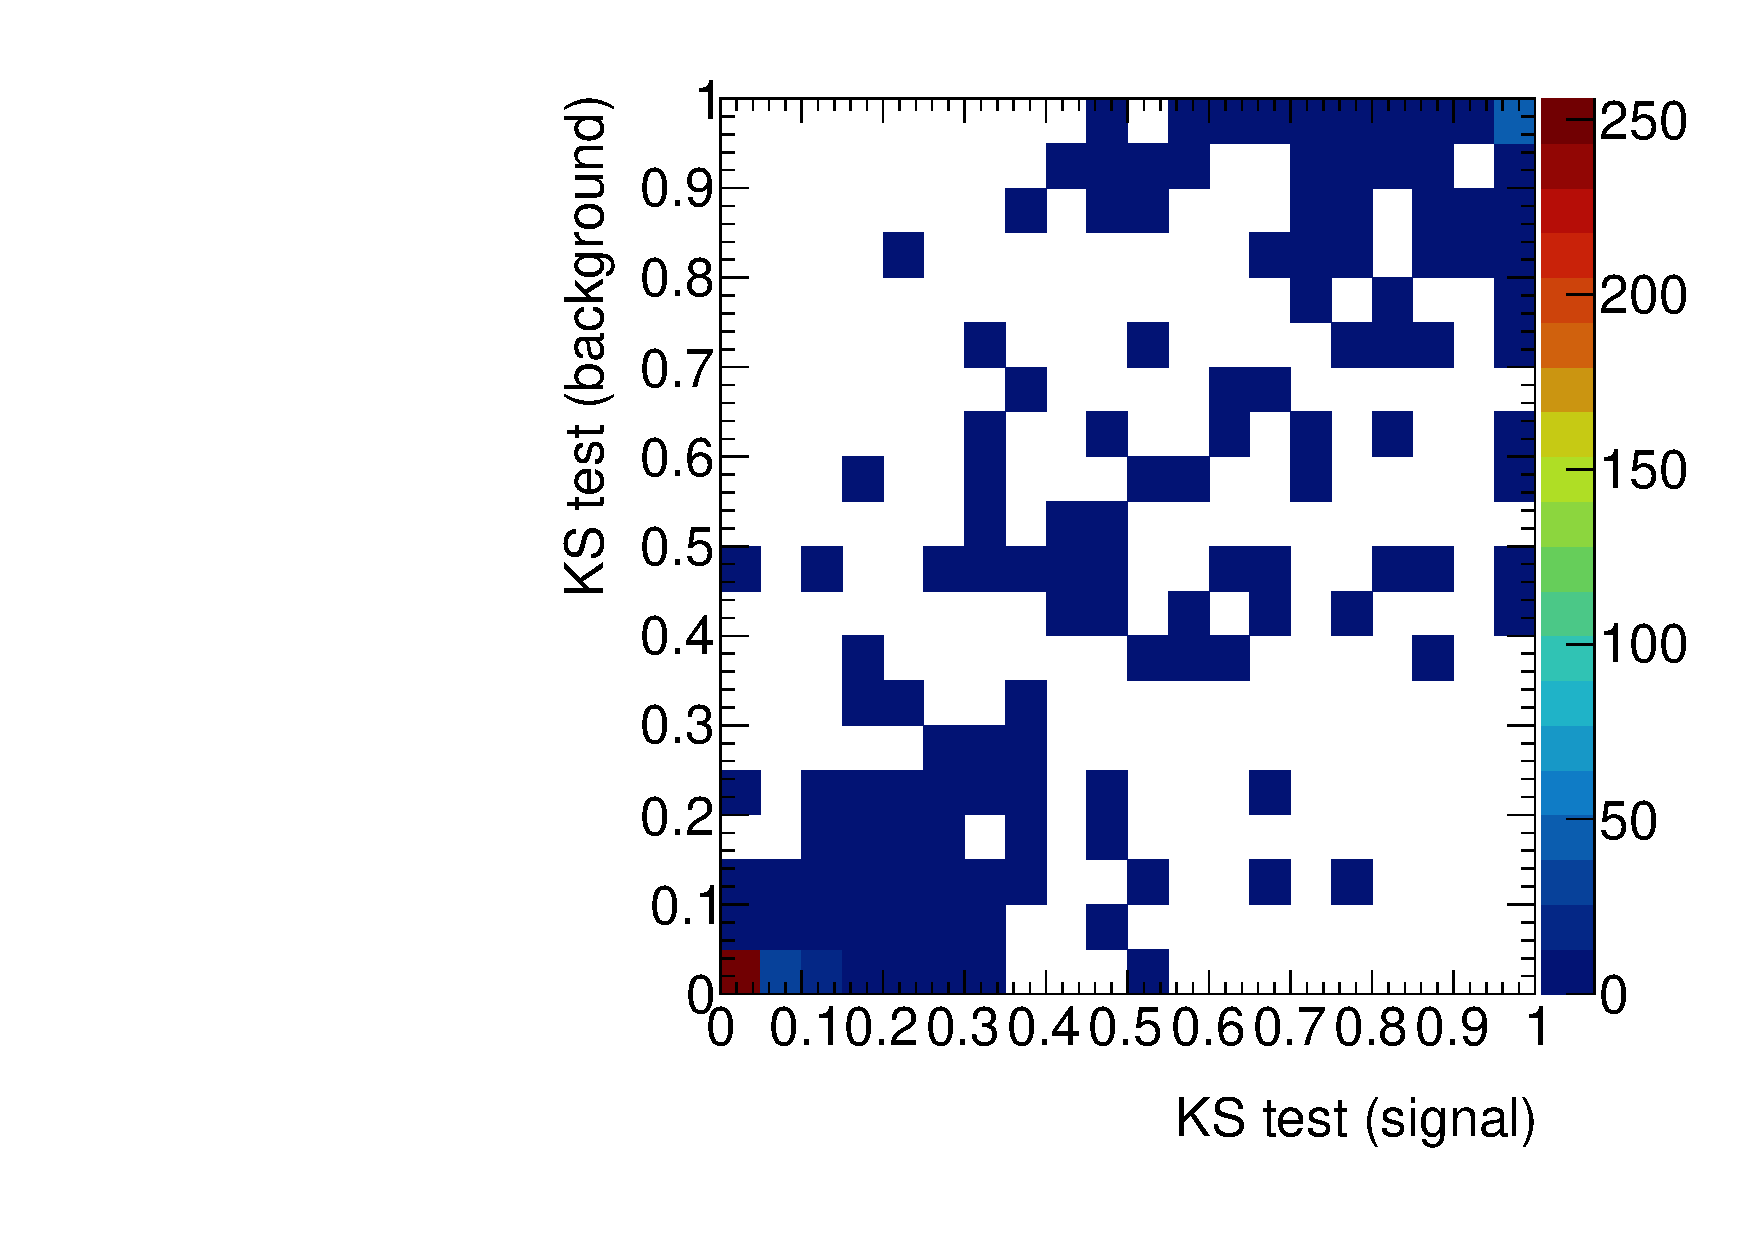
\includegraphics[width=\textwidth]{./plots/mva/scan/BOOST_SF_ks_test_sig_vs_bkg.pdf}
        \caption{Boosted SF}
    \end{subfigure}
    \begin{subfigure}[t]{0.45\textwidth}
        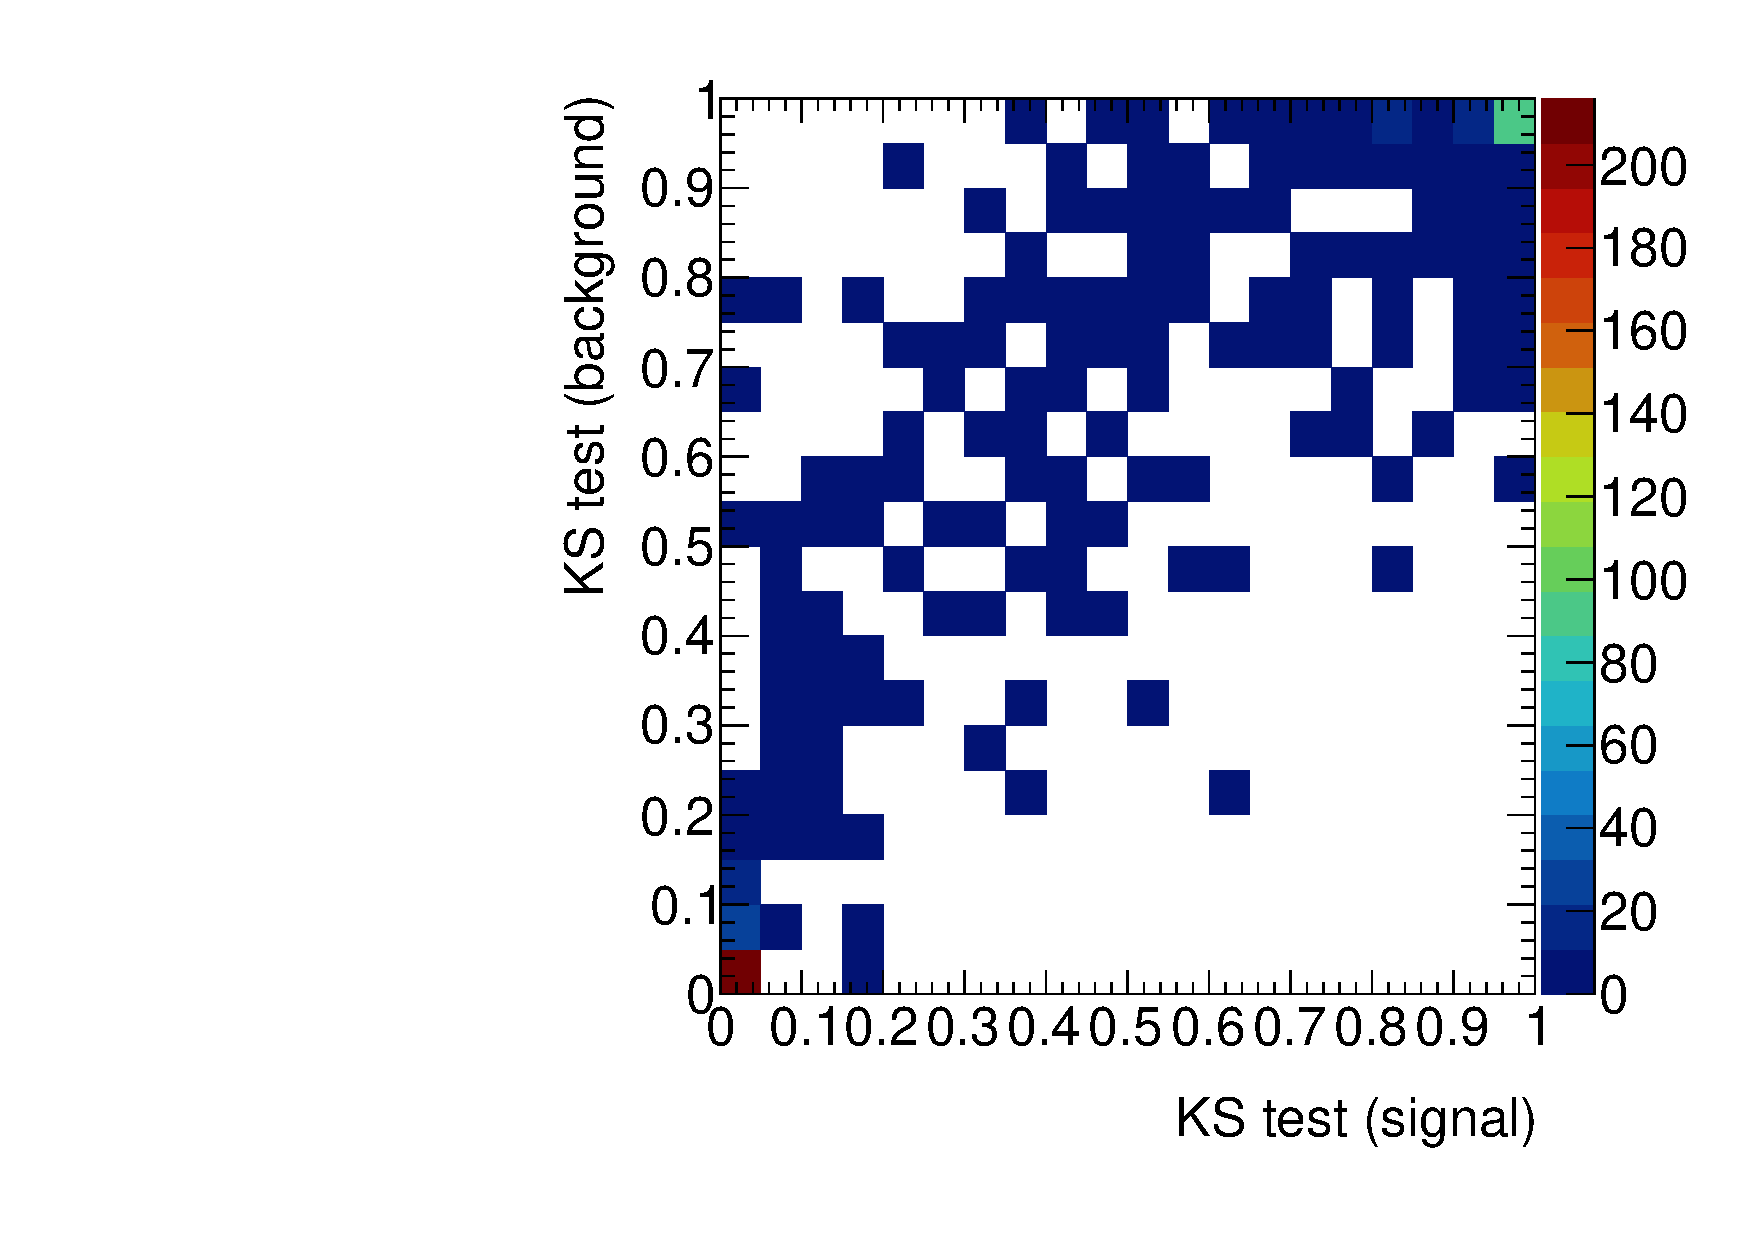
\includegraphics[width=\textwidth]{./plots/mva/scan/BOOST_DF_ks_test_sig_vs_bkg.pdf}
        \caption{Boosted DF}
    \end{subfigure}
    \caption{Correlation plots of the KS-test propability between the BDT output on the training and validaiton set for the signal and background distribution.}~\label{fig:mva:scan:kstest}
\end{figure}


\section{Variable Rankings}

\begin{table}[htpb]
    \centering
    \caption{Variable ranking for the final BDT in the VBF SF region calculated by averaging over the individual
             variable rankings of the $10$ BDTs from the $k$-fold cross-validation.}\label{tab:mva:variables:ranking:VBFSF}
    \begin{tabular}{rlcc}
        \toprule
        Rank & Observable & Mean Variable Separation & Standard Deviation \\ \midrule
        1 & $\drll$ & 0.212 & 0.016 \\
        2 & $\mmc$ & 0.178 & 0.015 \\
        3 & $\min \Delta R (\ell\ell, \text{jets})$ & 0.154 & 0.014 \\
        4 & $\mjj$ & 0.130 & 0.014 \\
        5 & $\min \Delta R (\ell_2, \text{jets})$ & 0.098 & 0.018 \\
        6 & $n_\text{jets}$ & 0.089 & 0.007 \\
        7 & $\etmiss \phi$ centrality & 0.080 & 0.011 \\
        8 & $\pt^\text{total}$ & 0.053 & 0.025 \\
        9 & $\etmiss$ & 0.005 & 0.007 \\
        \bottomrule
    \end{tabular}
\end{table}

\begin{table}[htpb]
    \centering
    \caption{Variable ranking for the final BDT in the VBF SF region calculated by averaging over the individual
             variable rankings of the $10$ BDTs from the $k$-fold cross-validation.}\label{tab:mva:variables:ranking:VBFDF}
    \begin{tabular}{rlcc}
        \toprule
        Rank & Observable & Mean Variable Separation & Standard Deviation \\ \midrule
        1 & $\drll$ & 0.180 & 0.009 \\
        2 & $\min \Delta R (\ell\ell, \text{jets})$ & 0.165 & 0.009 \\
        3 & $\etmiss \phi$ centrality & 0.144 & 0.009 \\
        4 & $\mmc$ & 0.132 & 0.014 \\
        5 & $\min \Delta R (\ell_2, \text{jets})$ & 0.129 & 0.010 \\
        6 & $\mjj$ & 0.112 & 0.011 \\
        7 & $\pt^\text{total}$ & 0.090 & 0.017 \\
        8 & $n_\text{jets}$ & 0.048 & 0.009 \\
        \bottomrule
    \end{tabular}
\end{table}
\begin{table}[htpb]
    \centering
    \caption{Variable ranking for the final BDT in the VBF SF region calculated by averaging over the individual
             variable rankings of the $10$ BDTs from the $k$-fold cross-validation.}\label{tab:mva:variables:ranking:BOOSTSF}
    \begin{tabular}{rlcc}
        \toprule
        Rank & Observable & Mean Variable Separation & Standard Deviation \\ \midrule
        1 & $\mmc$ & 0.446 & 0.038 \\
        2 & $\drll$ & 0.238 & 0.031 \\
        3 & $\mll$ & 0.227 & 0.019 \\
        4 & $\etmiss$ & 0.089 & 0.017 \\
        \bottomrule
    \end{tabular}
\end{table}
\begin{table}[htpb]
    \centering
    \caption{Variable ranking for the final BDT in the VBF SF region calculated by averaging over the individual
             variable rankings of the $10$ BDTs from the $k$-fold cross-validation.}\label{tab:mva:variables:ranking:BOOSTSF}
    \begin{tabular}{rlcc}
        \toprule
        Rank & Observable & Mean Variable Separation & Standard Deviation \\ \midrule
        1 & $\mmc$ & 0.263 & 0.007 \\
        2 & $m_\text{T}^{\ell_0}$ & 0.115 & 0.009 \\
        3 & $\min \Delta R (\ell\ell, \text{jets})$ & 0.107 & 0.007 \\
        4 & $\mll$ & 0.107 & 0.010 \\
        5 & $m_{\tau\tau,\text{j}_1}$ & 0.097 & 0.006 \\
        6 & $\drll$ & 0.085 & 0.009 \\
        7 & $\etmiss / \pt^{\ell_2}$ & 0.078 & 0.015 \\
        8 & Sphericity & 0.075 & 0.004 \\
        9 & $\eta_{\ell_1}$ & 0.074 & 0.009 \\
        \bottomrule
    \end{tabular}
\end{table}

\section{Correlations of input variables}\label{app:mva:correlation_inputvars}

\begin{figure}[htb]
    \centering
    \begin{subfigure}[t]{0.7\textwidth}
        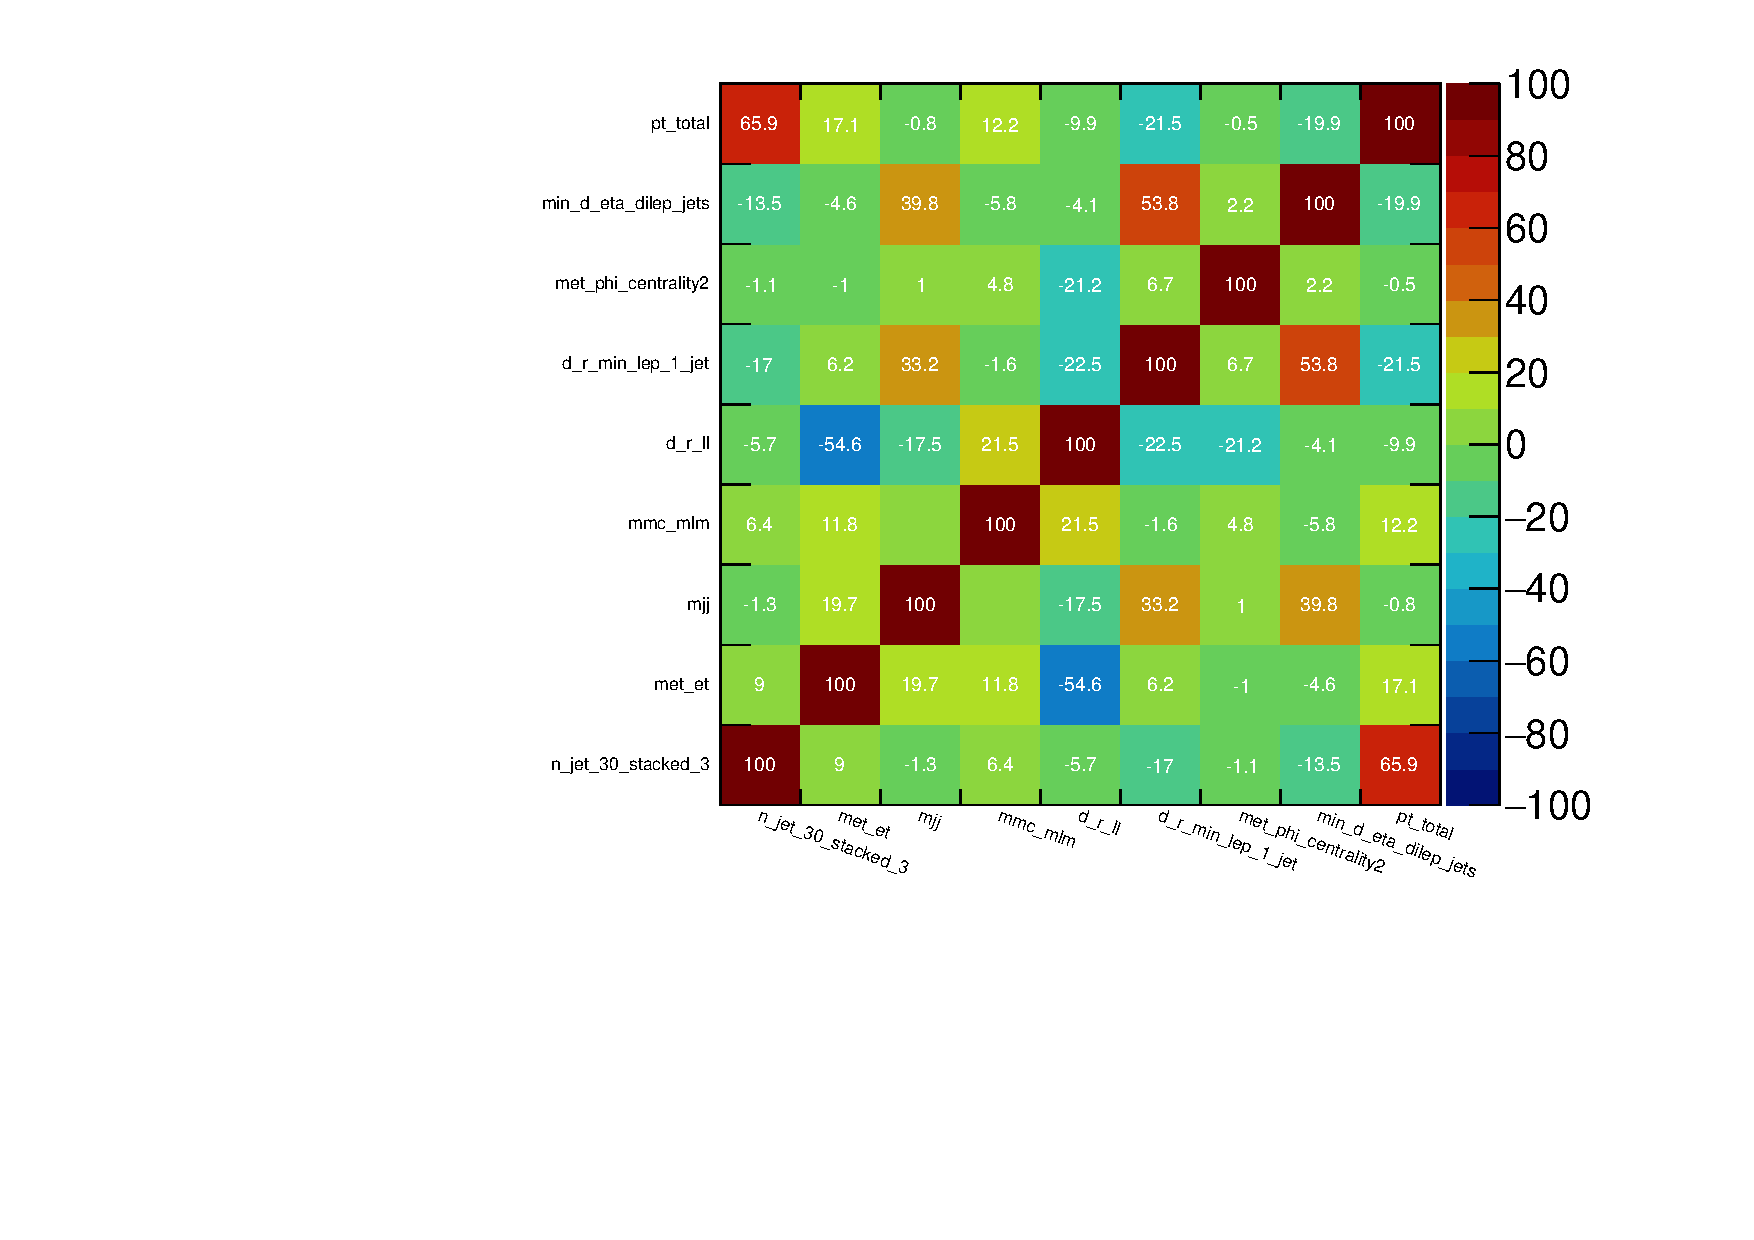
\includegraphics[width=\textwidth]{./plots/mva/variable_reduction/VBF_SF_CorrelationMatrixS.pdf}
        \caption{Signal.}
    \end{subfigure}
    \begin{subfigure}[t]{0.7\textwidth}
        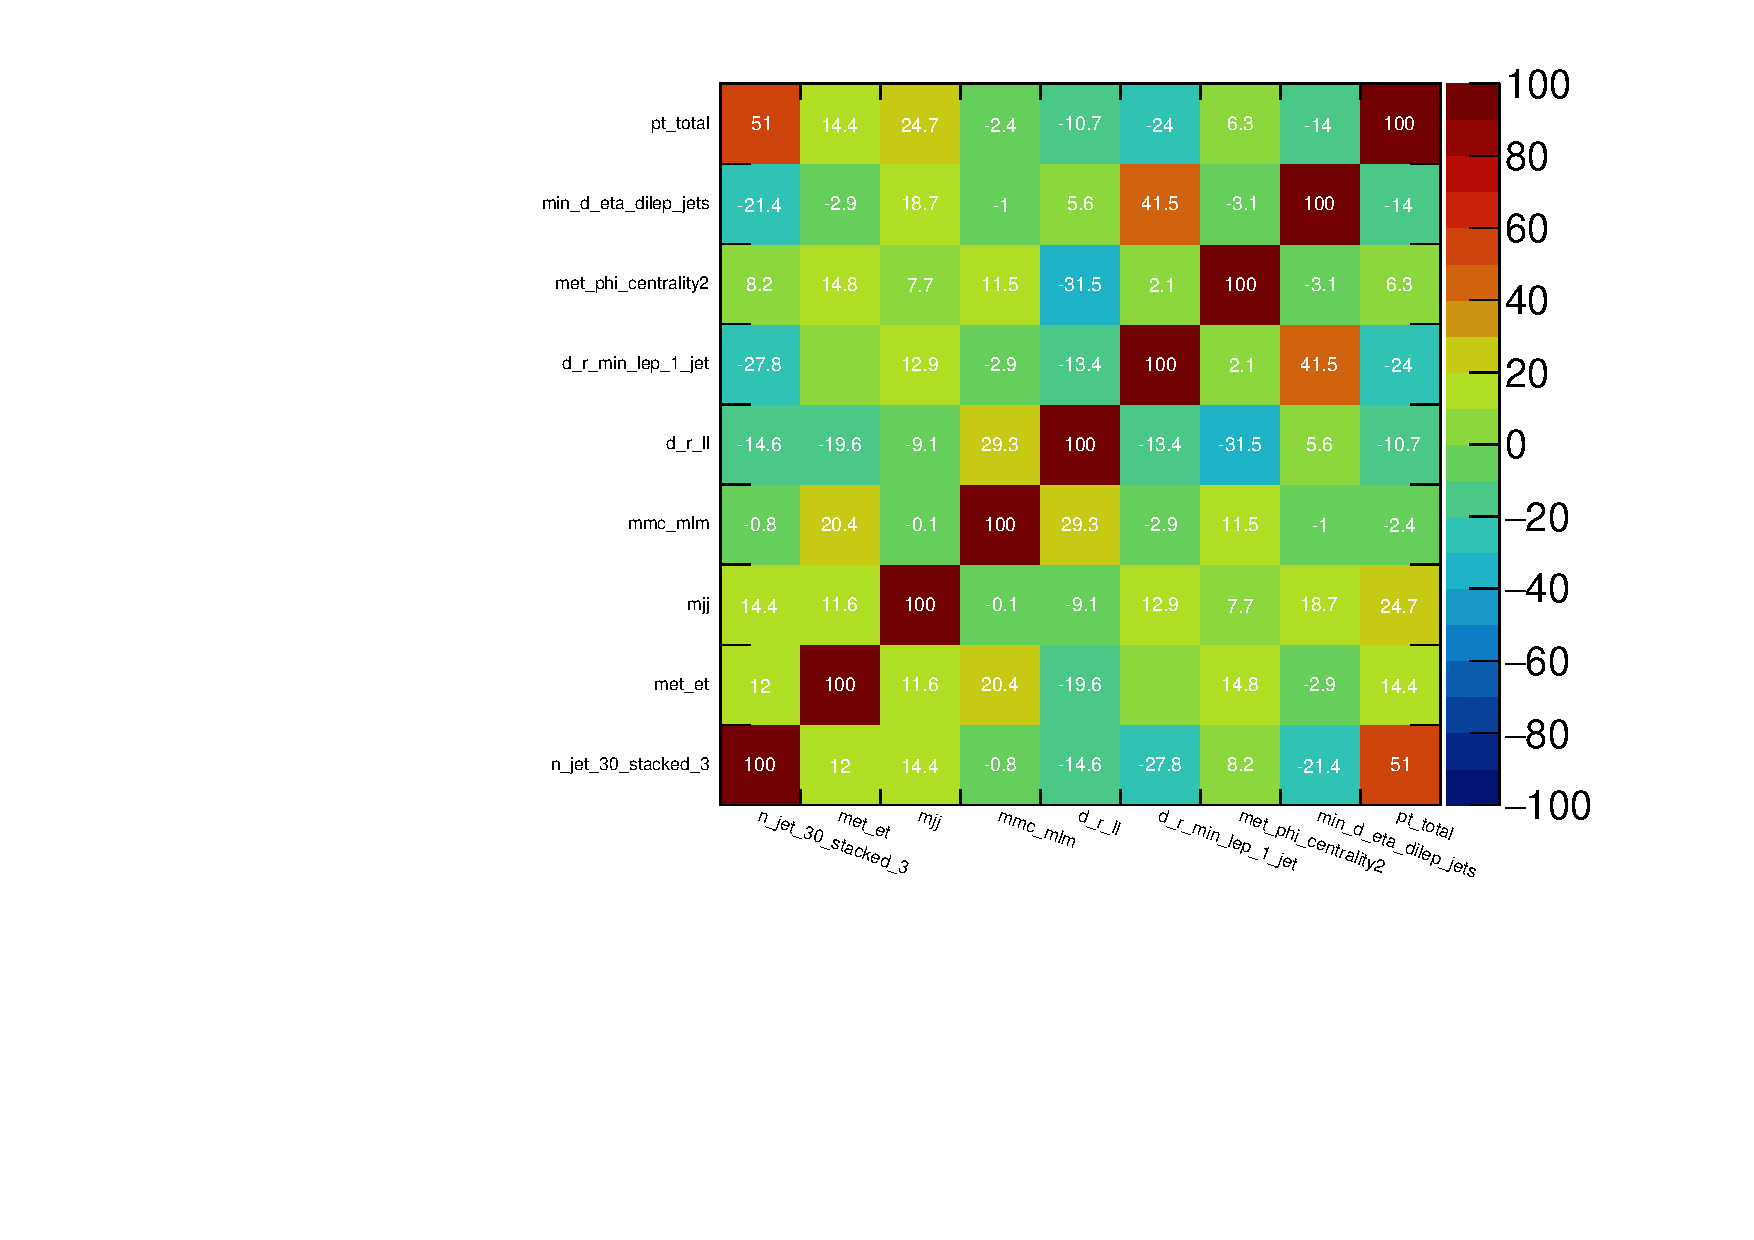
\includegraphics[width=\textwidth]{./plots/mva/variable_reduction/VBF_SF_CorrelationMatrixB.pdf}
        \caption{Background}
    \end{subfigure}
    \caption{Correlations of the input variables for the BDTs in the VBF SF category for signal and background events.}\label{fig:mva:variables:correlationsb:vbfsf}
\end{figure}

\begin{figure}[htb]
    \centering
    \begin{subfigure}[t]{0.7\textwidth}
        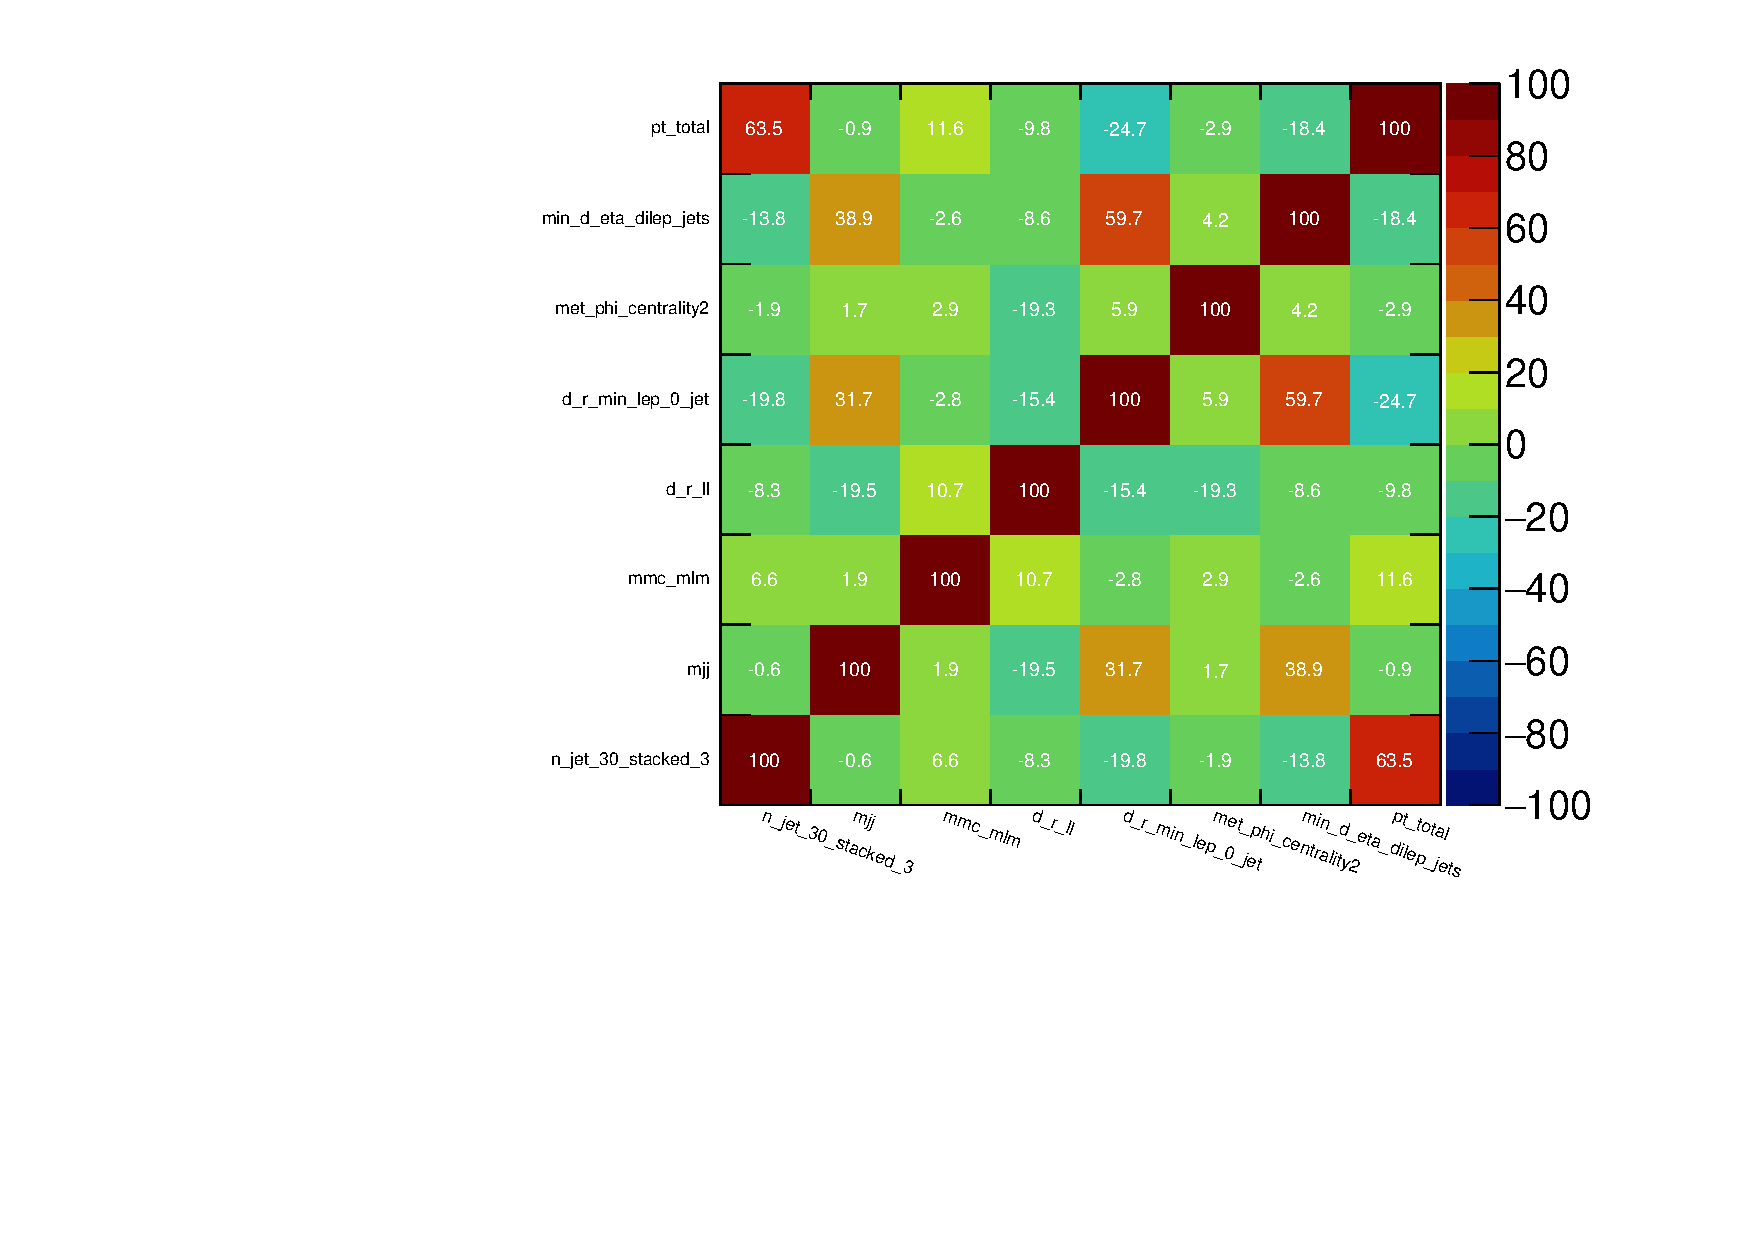
\includegraphics[width=\textwidth]{./plots/mva/variable_reduction/VBF_DF_CorrelationMatrixS.pdf}
        \caption{Signal.}
    \end{subfigure}
    \begin{subfigure}[t]{0.7\textwidth}
        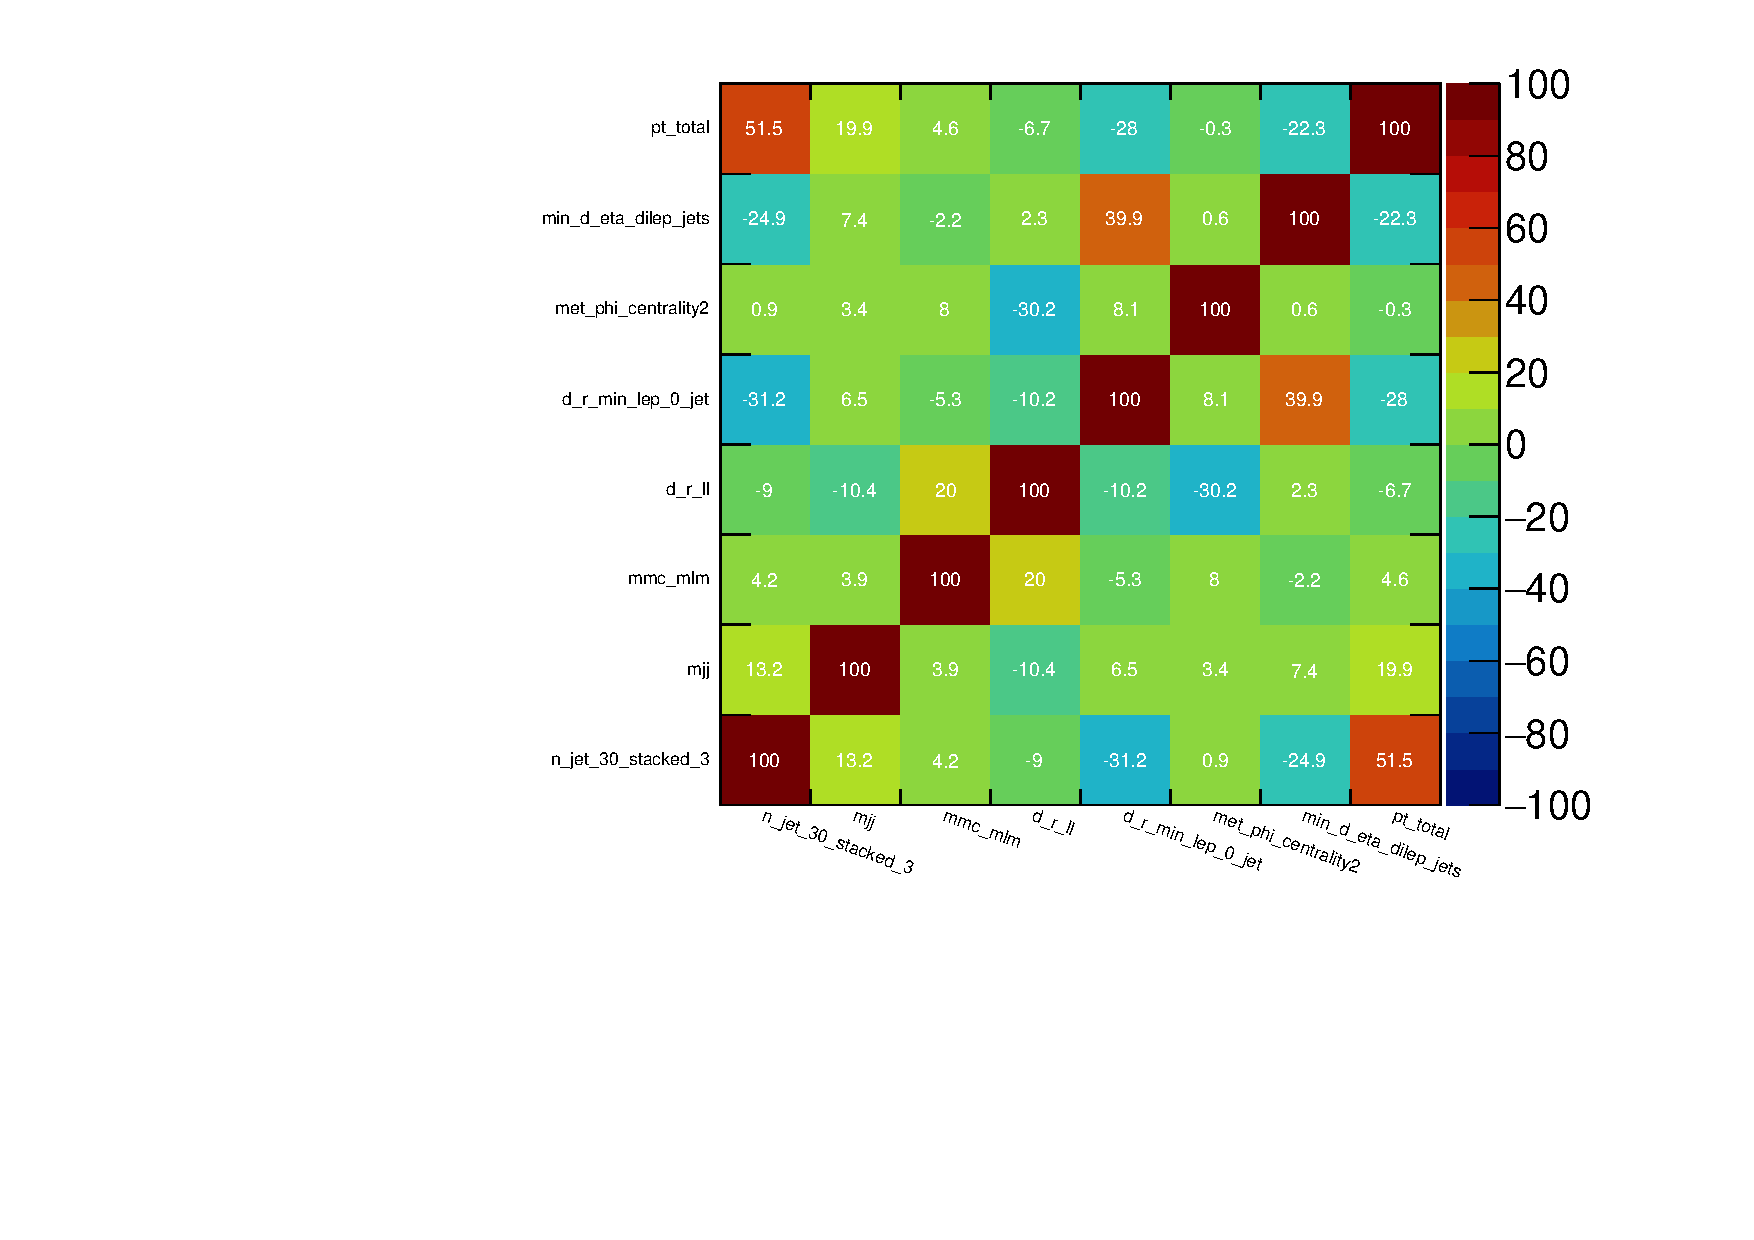
\includegraphics[width=\textwidth]{./plots/mva/variable_reduction/VBF_DF_CorrelationMatrixB.pdf}
        \caption{Background}
    \end{subfigure}
    \caption{Correlations of the input variables for the BDTs in the VBF DF category for signal and background events.}\label{fig:mva:variables:correlationsb:vbfdf}
\end{figure}

\begin{figure}[htb]
    \centering
    \begin{subfigure}[t]{0.7\textwidth}
        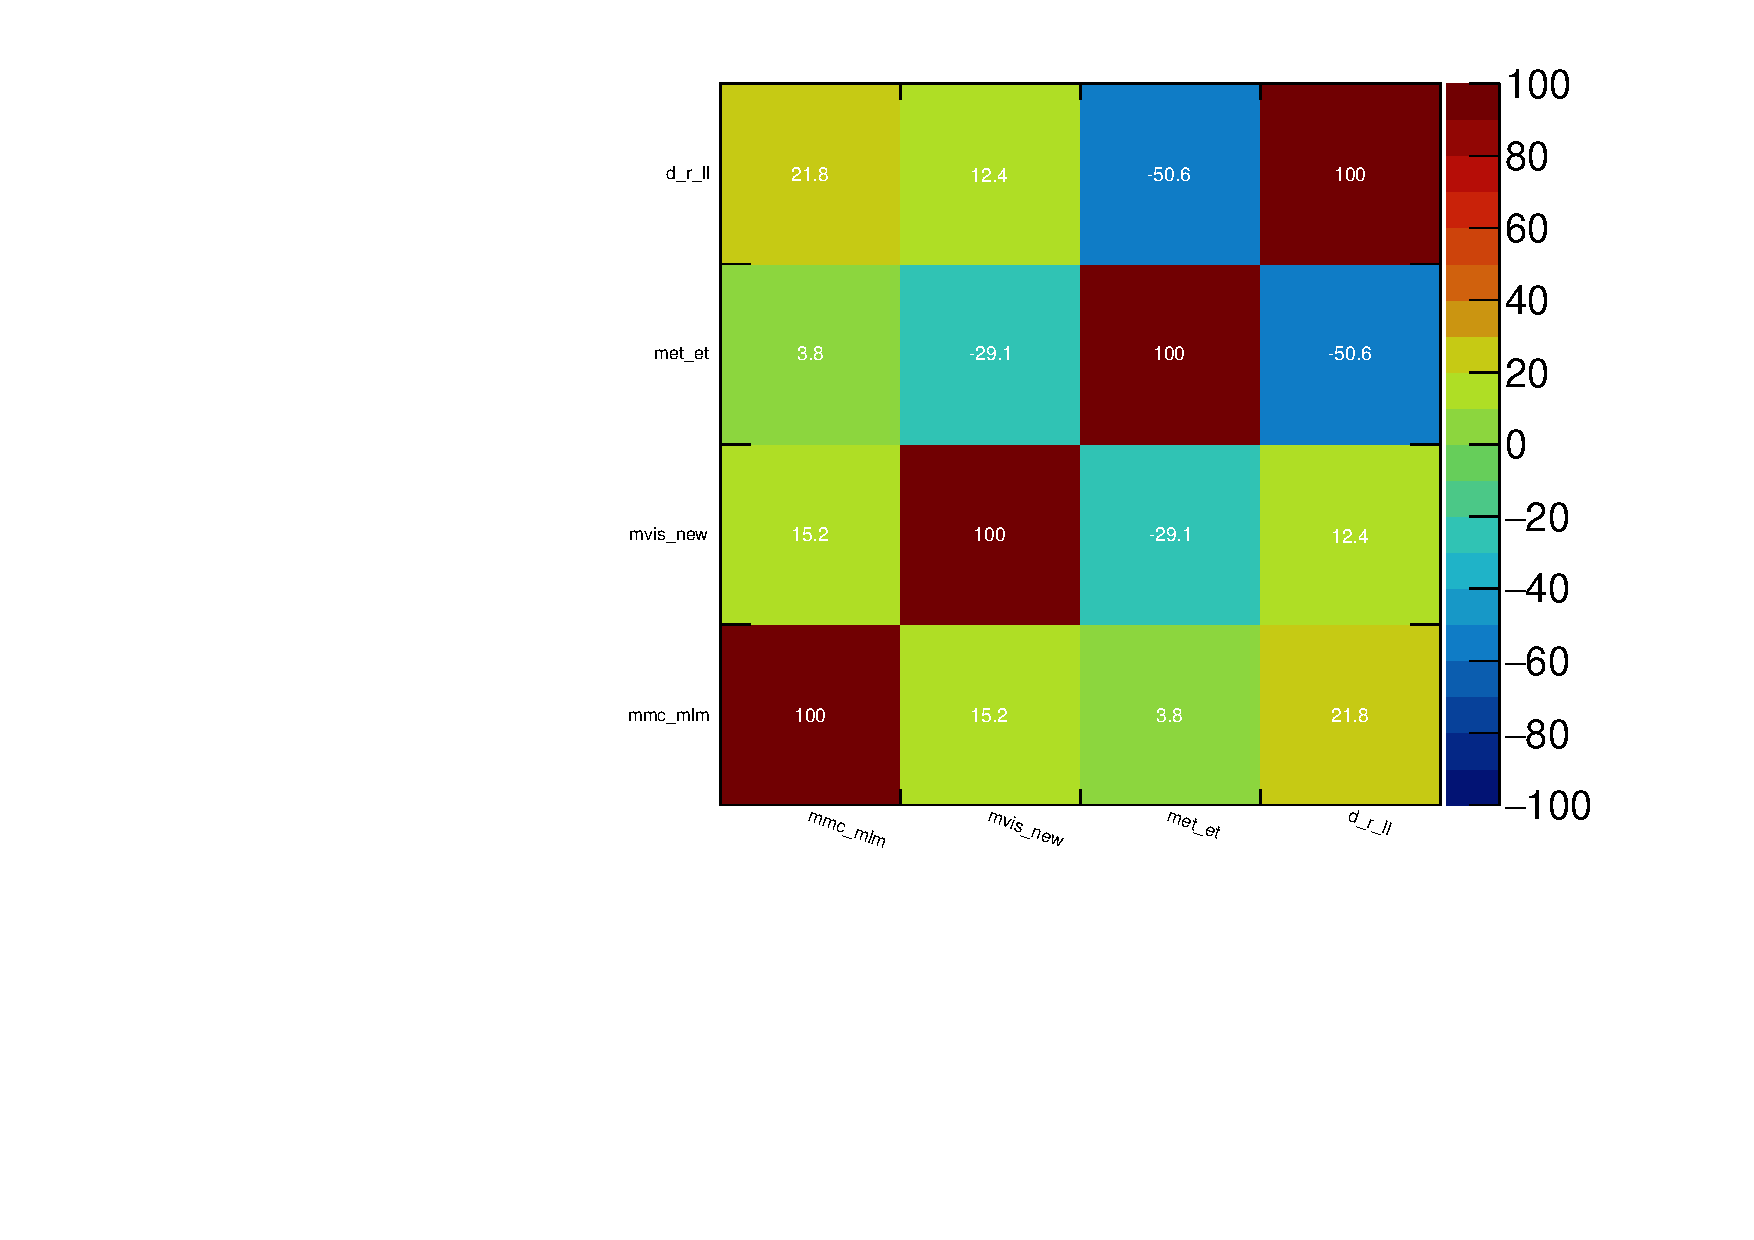
\includegraphics[width=\textwidth]{./plots/mva/variable_reduction/BOOST_SF_CorrelationMatrixS.pdf}
        \caption{Signal.}
    \end{subfigure}
    \begin{subfigure}[t]{0.7\textwidth}
        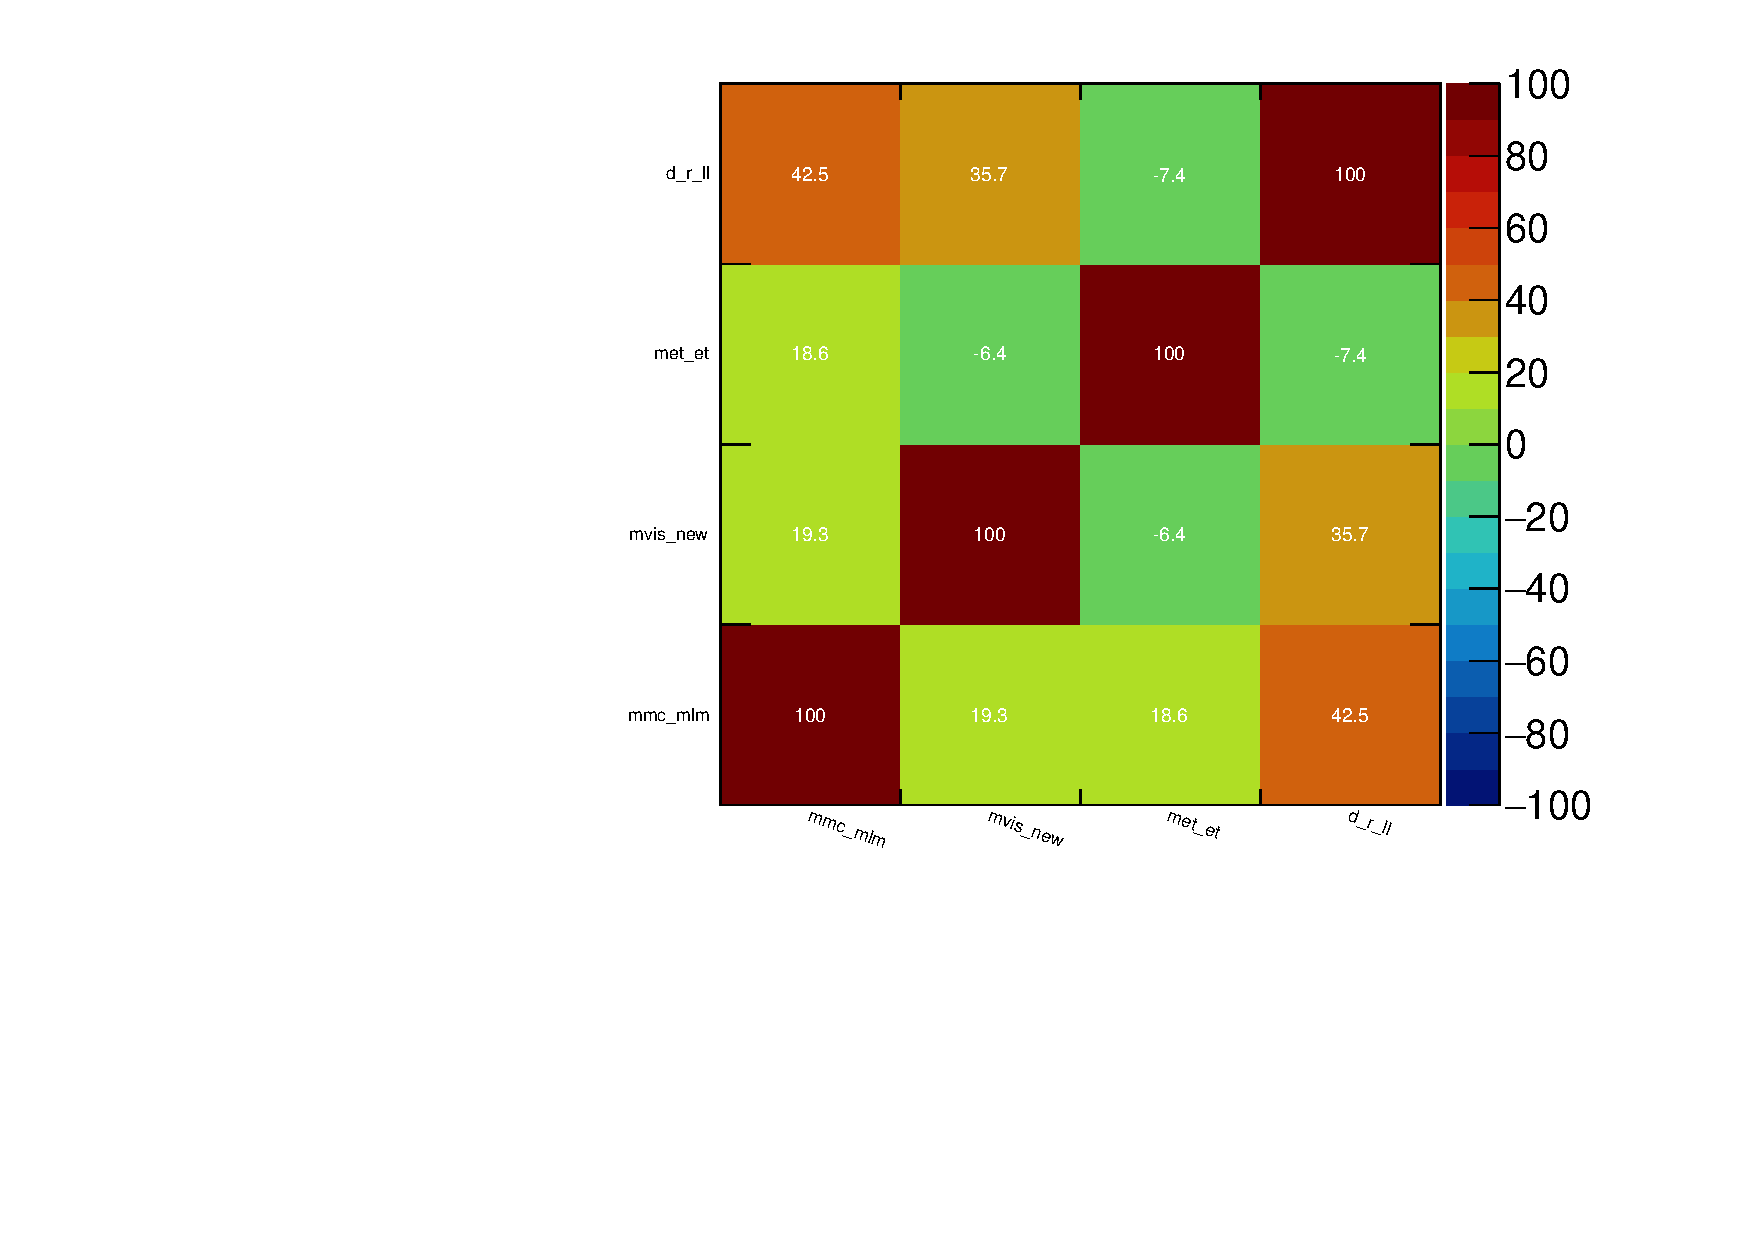
\includegraphics[width=\textwidth]{./plots/mva/variable_reduction/BOOST_SF_CorrelationMatrixB.pdf}
        \caption{Background}
    \end{subfigure}
    \caption{Correlations of the input variables for the BDTs in the boosted SF category for signal and background events.}\label{fig:mva:variables:correlationsb:boostsf}
\end{figure}\begin{figure}[htb]
    \centering
    \begin{subfigure}[t]{0.7\textwidth}
        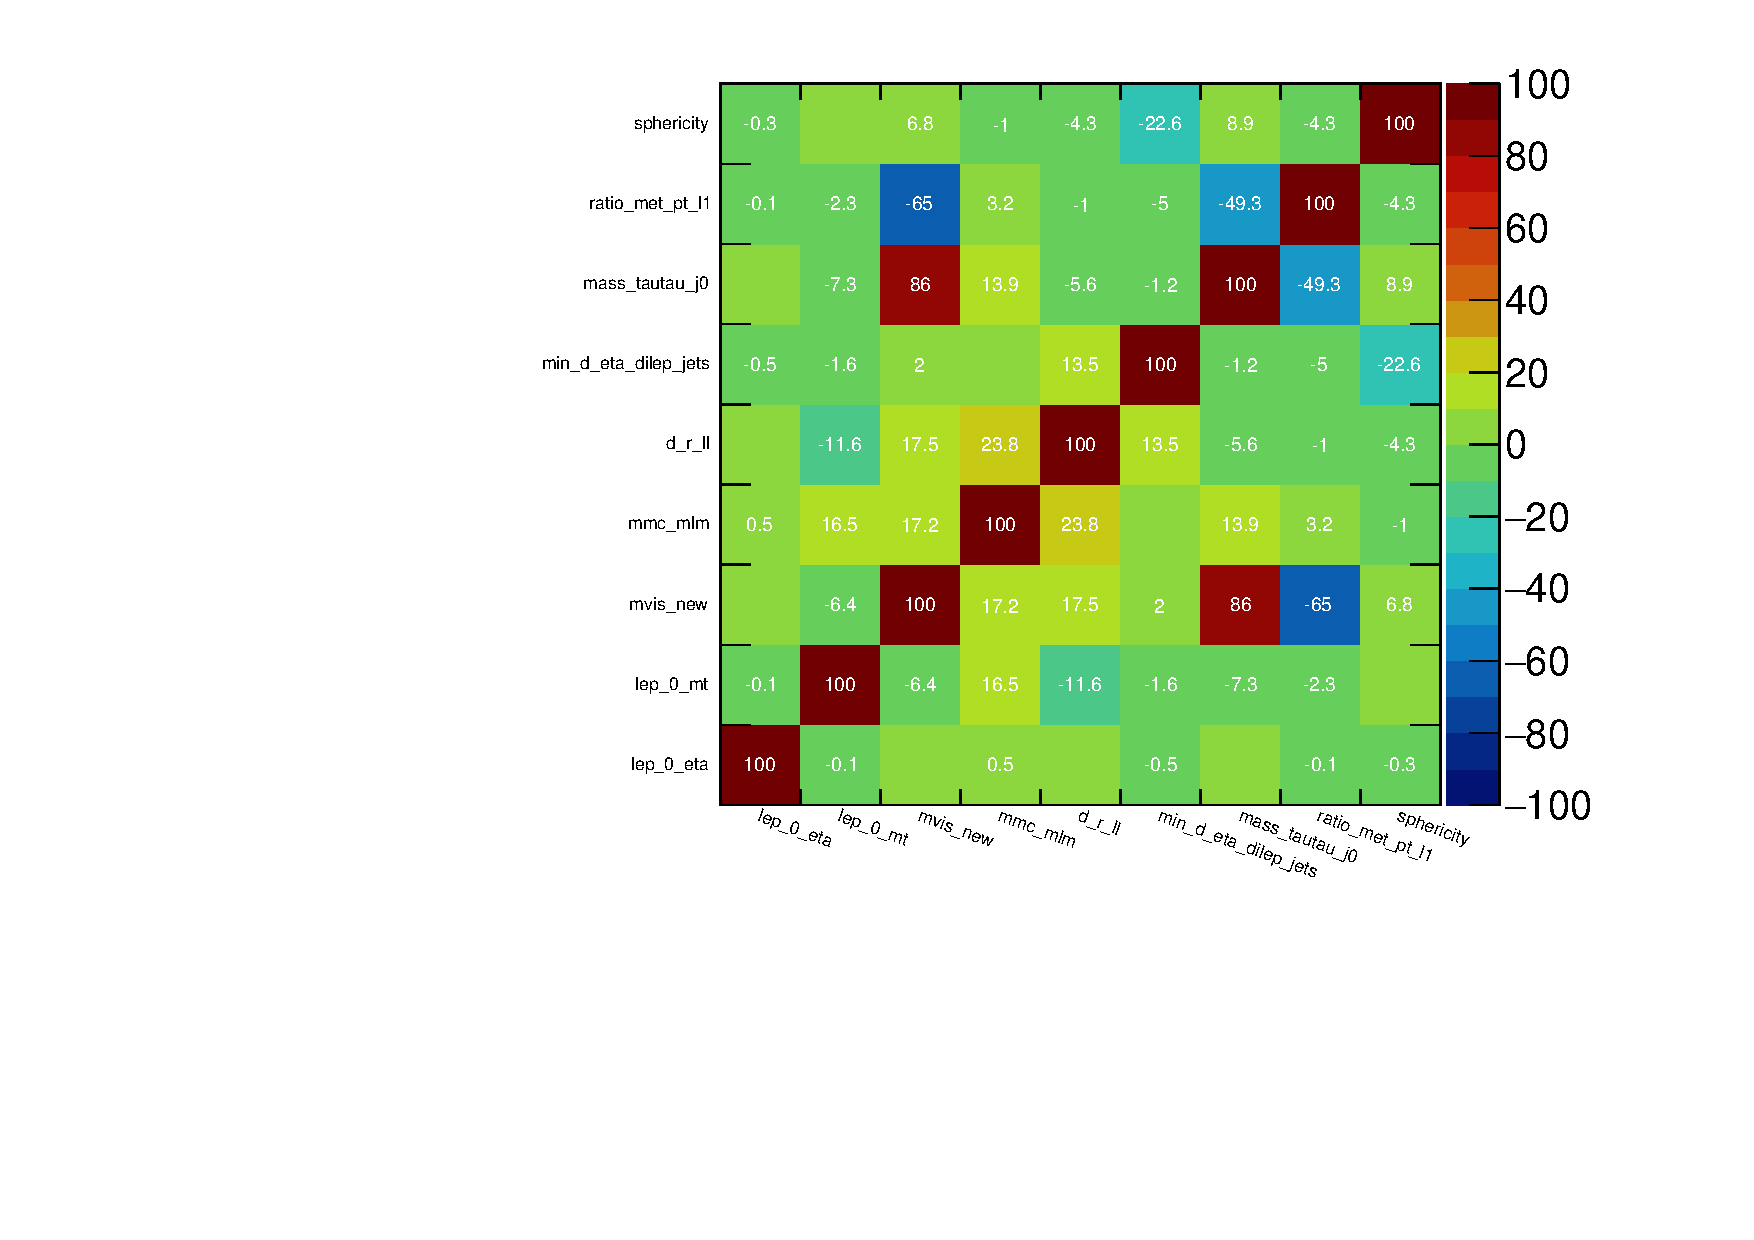
\includegraphics[width=\textwidth]{./plots/mva/variable_reduction/BOOST_DF_CorrelationMatrixS.pdf}
        \caption{Signal.}
    \end{subfigure}
    \begin{subfigure}[t]{0.7\textwidth}
        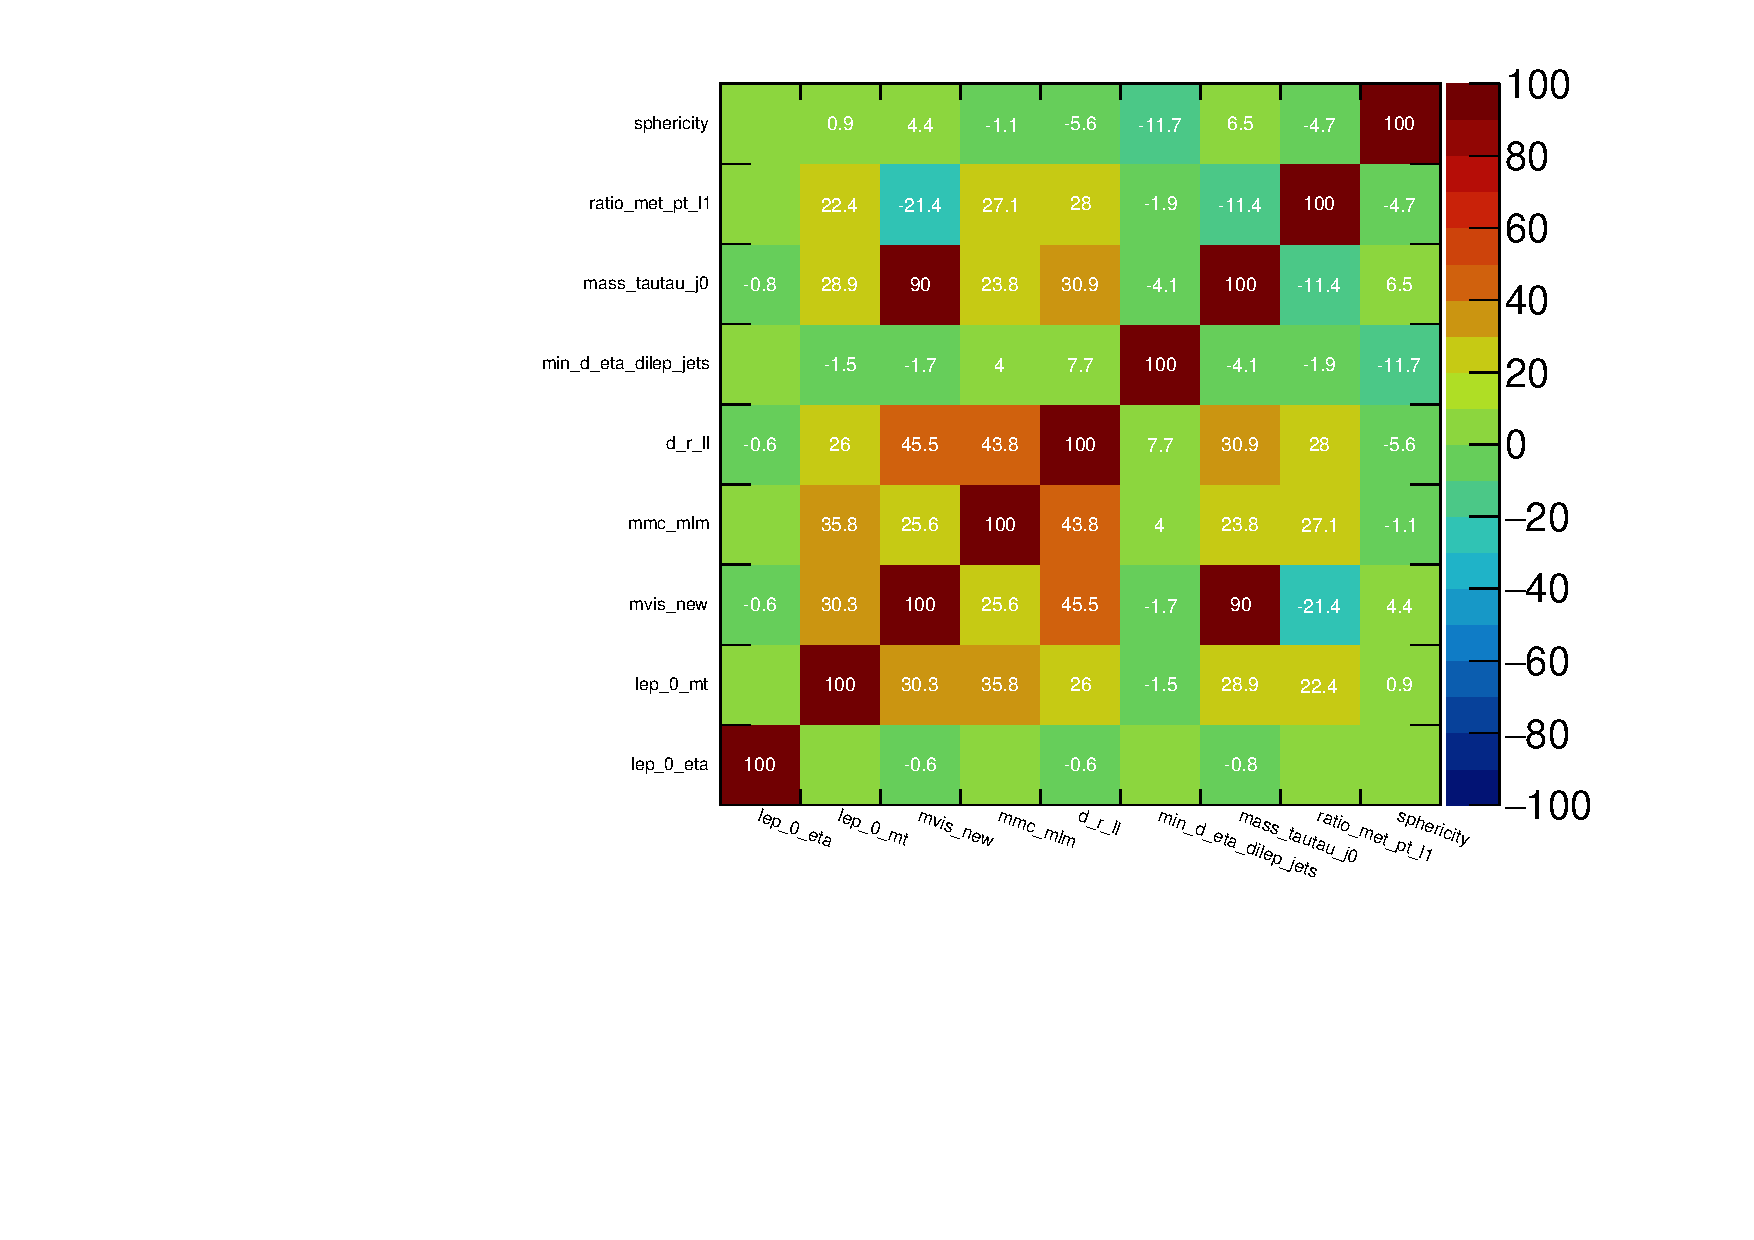
\includegraphics[width=\textwidth]{./plots/mva/variable_reduction/BOOST_DF_CorrelationMatrixB.pdf}
        \caption{Background}
    \end{subfigure}
    \caption{Correlations of the input variables for the BDTs in the boosted DF category for signal and background events.}\label{fig:mva:variables:correlationsb:boostdf}
\end{figure}
